% !TEX root = ../om_ts_002.tex


\begin{frame} % frame name
	
	\videotitle{Unit root tests: ADF test}
	
\end{frame}




\begin{frame}{ADF test: Plan}
	\begin{itemize}[<+->]
		\item Test assumptions
		\item Test algorithm
		\item Three variations of the test
	\end{itemize}
	
\end{frame}




\begin{frame}
	\frametitle{Why do we need an stationarity tests?}
	
	We want to answer the questions:
	\pause
	\begin{itemize}[<+->]
		\item Should the $ARMA$ model be used for $(y_t)$ or for $(\Delta y_t)$?
		\item How to include a constant in a model?
	\end{itemize}
	
	\pause
	Name "unit root test":
	\pause
	\[
	\Delta = 1 - L = P(L)
	\]
	The equation $1 - \ell = 0$ has a root $\ell =1$
	
\end{frame}


\begin{frame}
	\frametitle{ADF test}
	
	ADF — \alert{Augmented Dickey Fuller} test
	
	\pause
	Three variations of the test: without a constant, with a constant, with a trend
	
\end{frame}


\begin{frame}
	\frametitle{ADF with constant}
	\[
	\Delta y_t = c + \beta y_{t-1} + d_1 \Delta y_{t-1} + \ldots + d_p \Delta y_{t-p} + u_t,
	\]
	
	\pause
	
	\alert{$H_0$: $\beta = 0$}
	
	$\Delta y_t = m + x_t$;
	
	$(x_t)$ is a stationary $AR(p)$ process with $\E(x_t) = 0$;
	
	$y_t = y_0 + mt + \sum_{i=1}^t x_i$
	
	\pause
	
	\alert{$H_a$: $\beta < 0$}
	
	$(y_t)$ is a stationary $AR(p + 1)$ process
	
\end{frame}

\begin{frame}
	\frametitle{ADF with constant: $H_0$ and $H_a$}
	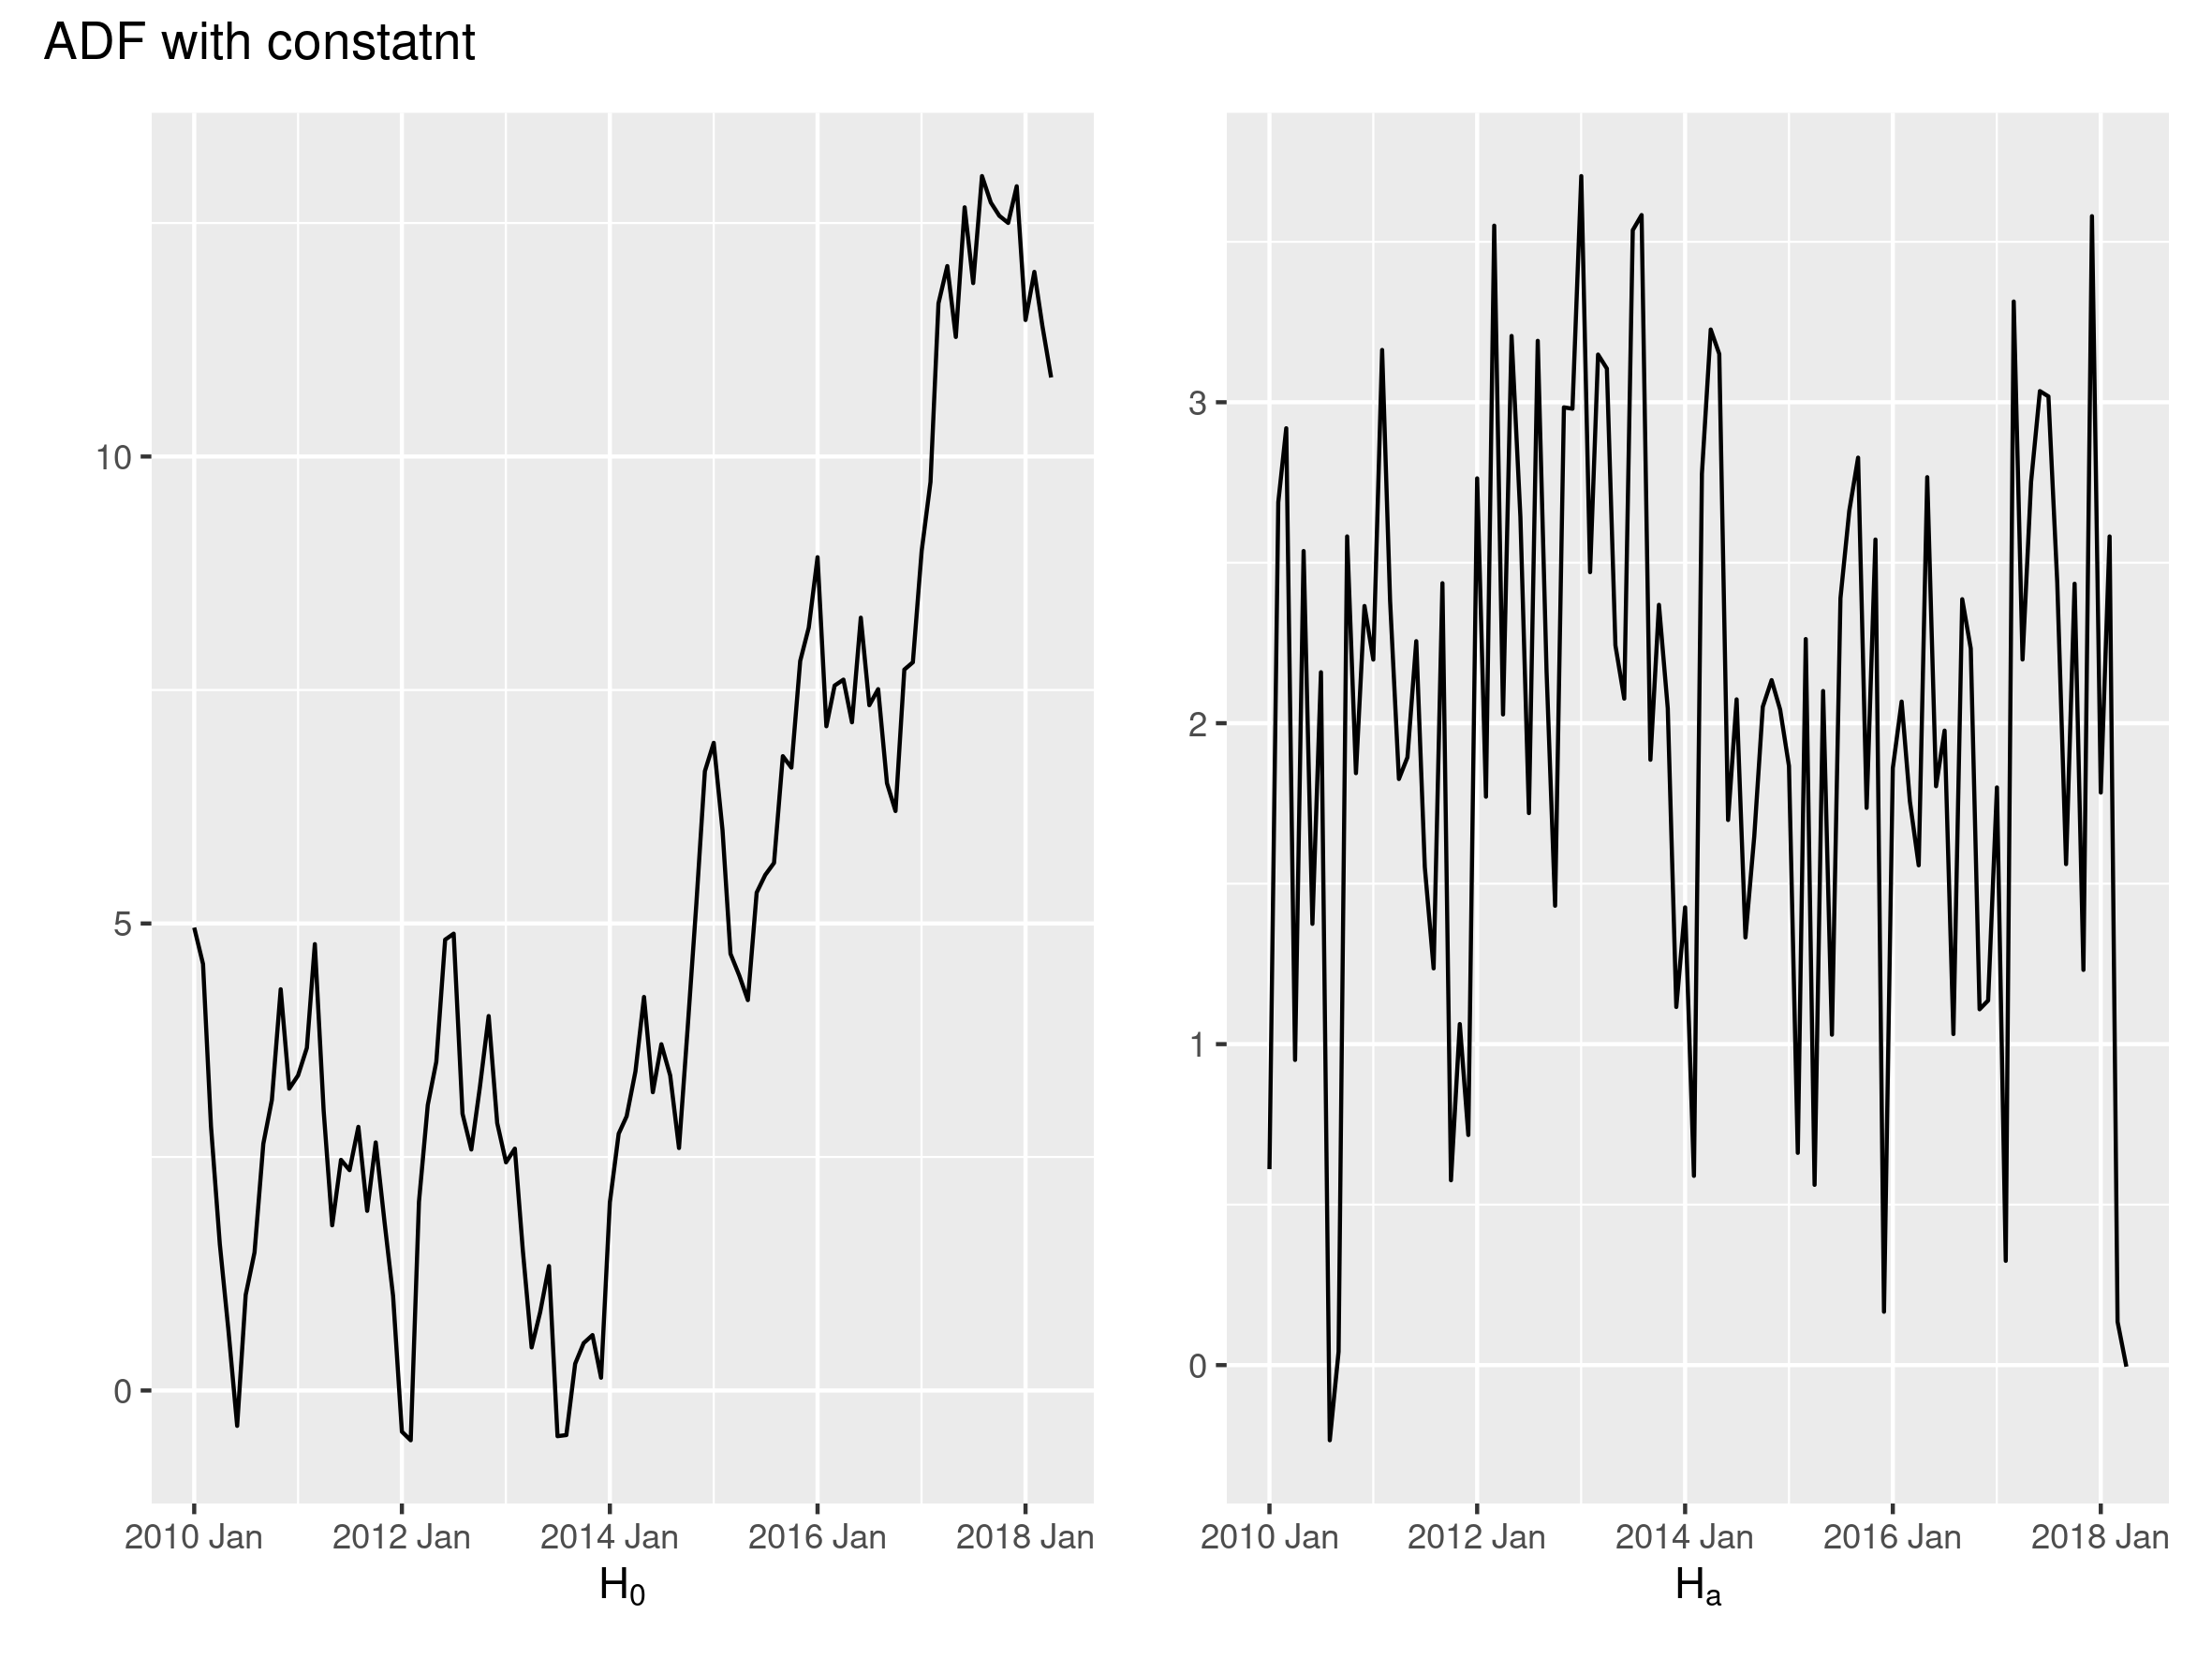
\includegraphics[width=\textwidth]{pictures/om_ts_06-046.png}
	
\end{frame}

\begin{frame}
	\frametitle{ADF with constant: algorithm}
	
	Step 1. Evaluate \alert{regression}
	\[
	\widehat{\Delta y_t} = \hat c + \hat \beta y_{t-1} + \hat d_1 \Delta y_{t-1} + \ldots + \hat d_p \Delta y_{t-p}
	\]
	
	\pause
	Step 2. Calculate the $t$-statistics using the \alert{classic formula}
	\[
	ADF = \frac{\hat \beta - 0}{se(\hat \beta)}
	\]
	
	\pause
	Under true $H_0$, the distribution of the $ADF$-statistic converges to the  special  \alert{DF distribution} with $DF^c$!
	
	\pause
	Step 3. We conclude:
	
	If $ADF < DF^c$ then $H_0$ is rejected
	
\end{frame}


\begin{frame}
	\frametitle{ADF without constant}
	\[
	\Delta y_t = \beta y_{t-1} + d_1 \Delta y_{t-1} + \ldots + d_p \Delta y_{t-p} + u_t,
	\]
	
	\pause
	
	\alert{$H_0$: $\beta = 0$}
	
	$(\Delta y_t)$ is a stationary $AR(p)$ process with $\E(\Delta y_t) = 0$;
	
	$y_t = y_0 + \sum_{i=1}^t \Delta y_i $
	
	\pause
	
	\alert{$H_a$: $\beta < 0$}
	
	$(y_t)$ is a stationary $AR(p + 1)$ process with $\E(y_t) = 0$;
	
	\pause
	
	The algorithm will have \alert{regression without a constant} and another distribution $DF^0$
	
\end{frame}


\begin{frame}
	\frametitle{ADF without constant: $H_0$ and $H_a$}
	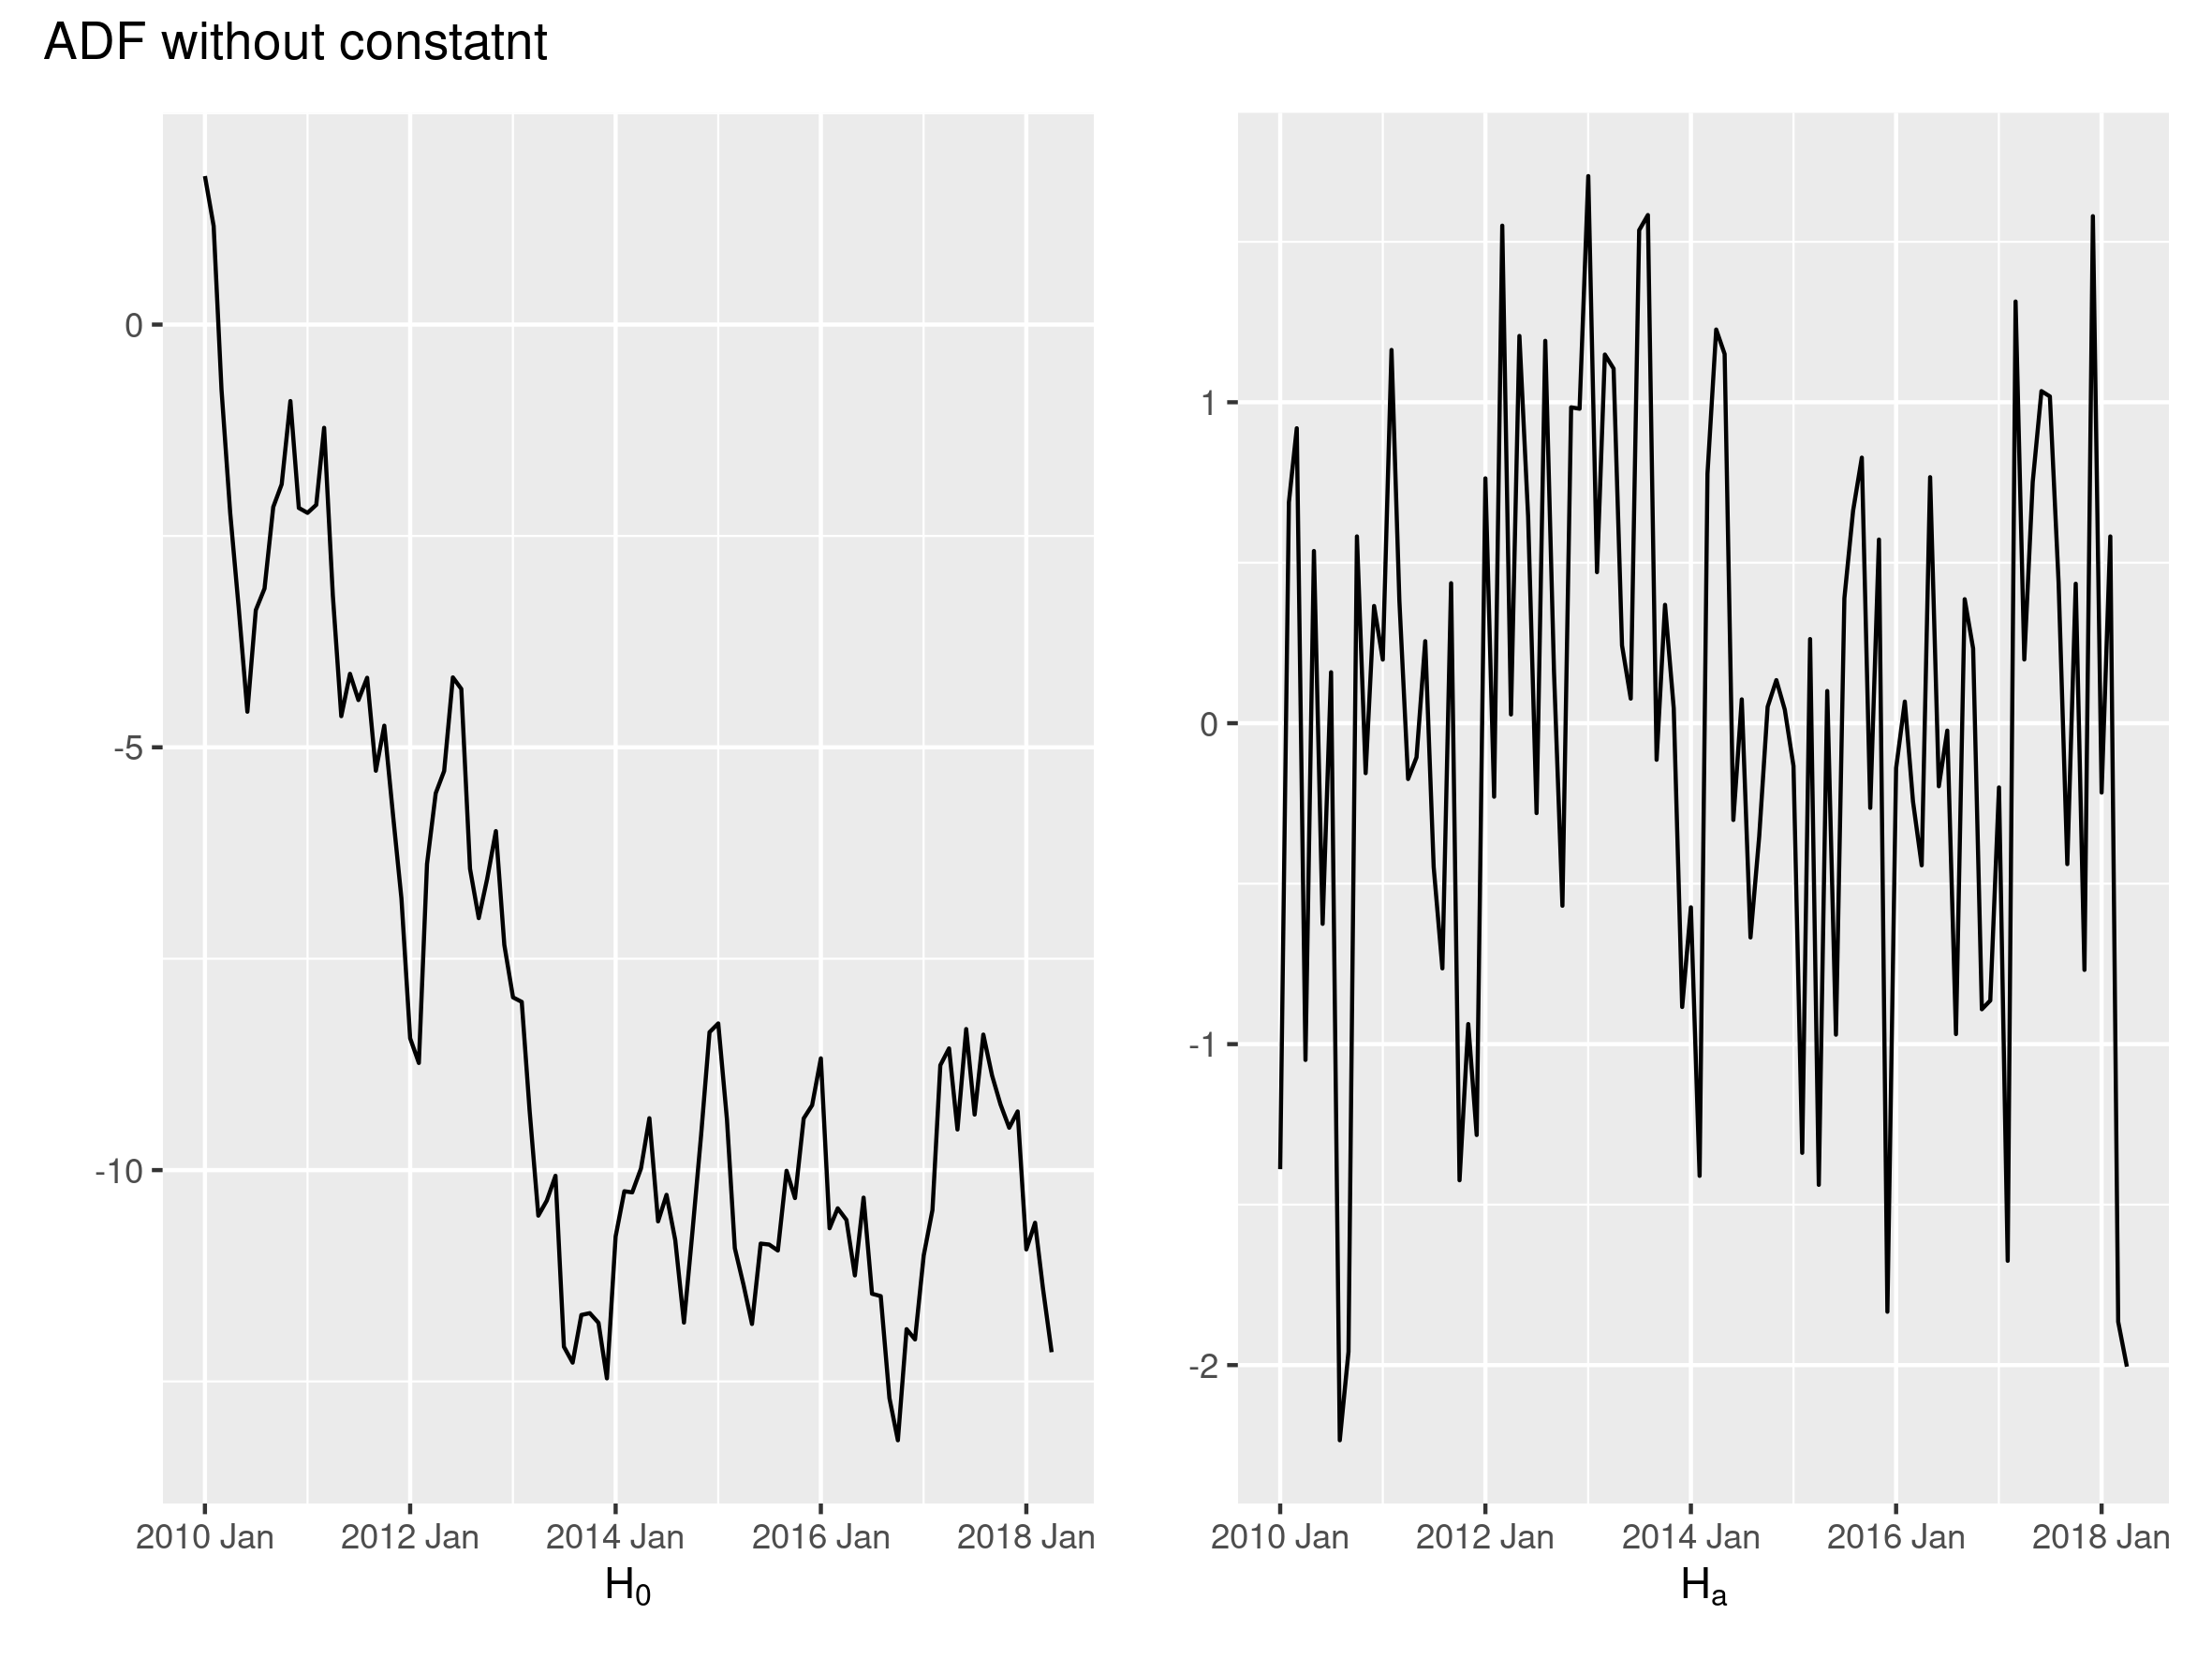
\includegraphics[width=\textwidth]{pictures/om_ts_06-055.png}
	
\end{frame}



\begin{frame}
	\frametitle{ADF with trend}
	\[
	\Delta y_t = c + g t + \beta y_{t-1} + d_1 \Delta y_{t-1} + \ldots + d_p \Delta y_{t-p} + u_t,
	\]
	
	\pause
	
	\alert{$H_0$: $\beta = 0$}
	
	$\Delta y_t = k_1 + k_2t + x_t$;
	
	$(x_t)$ is a stationary $AR(p)$ process with $\E(x_t) = 0$;
	
	$y_t = y_0 + m_1 t + m_2 t^2 + \sum_{i=1}^t x_i$
	
	\pause
	
	\alert{$H_a$: $\beta < 0$}
	
	$y_t = m_1 + m_2t + x_t$;
	
	$(x_t)$ is a stationary $AR(p + 1)$ process with $\E(x_t) = 0$;
	
	\pause
	
	The algorithm will have a regression \alert{with a constant and a trend} and another distribution $DF^{ct}$
	
\end{frame}


\begin{frame}
	\frametitle{ADF with trend: $H_0$ and $H_a$}
	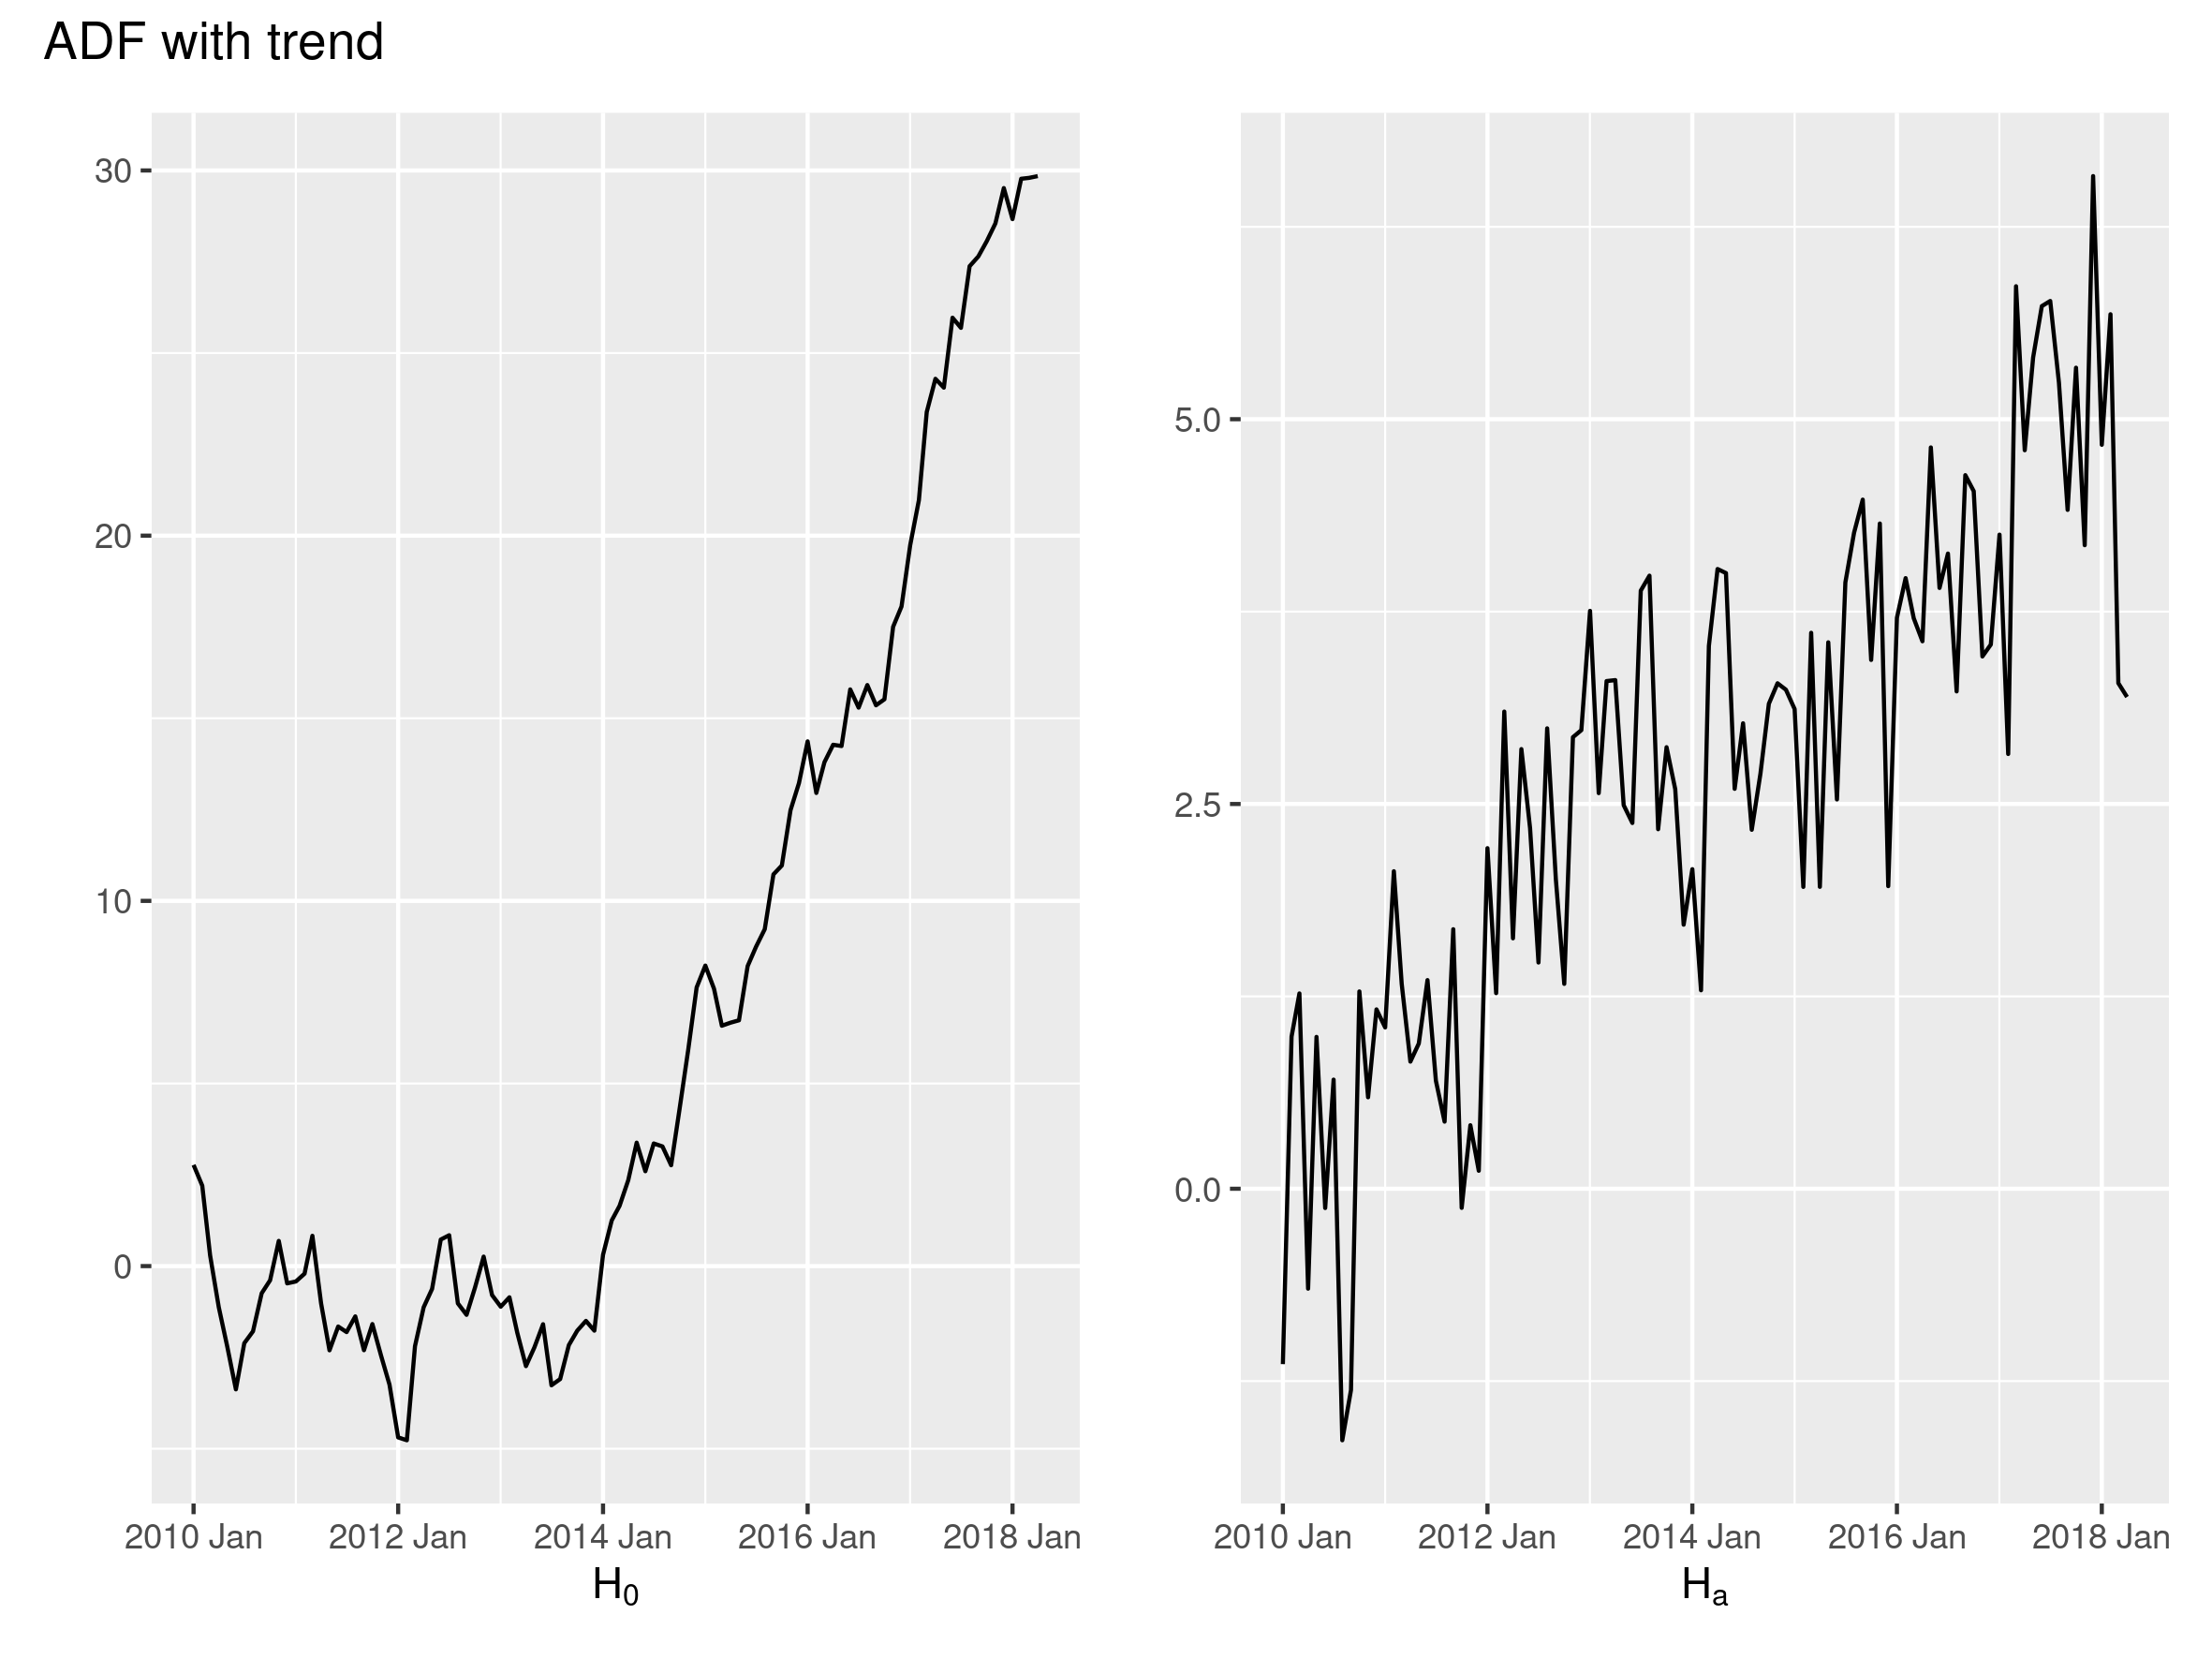
\includegraphics[width=\textwidth]{pictures/om_ts_06-060.png}
\end{frame}



\begin{frame}{$ADF$ test: Summary}
	
	\begin{itemize}[<+->]
		\item Applicable for making a decision about the transition to $\Delta y_t$
		\item Three variants of the ADF test with different assumptions		
	\end{itemize}
\end{frame}






\begin{frame} % frame name
	
	\videotitle{Unit root tests: KPSS test }
	
\end{frame}



\begin{frame}{KPSS test: Plan}
	\begin{itemize}[<+->]
		\item Long-term variance
		\item Prerequisites for the test
		\item Two variations of the test
	\end{itemize}
	
\end{frame}

\begin{frame}
	\frametitle{KPSS test}
	
	KPSS — \alert{Kwiatkowski–Phillips–Schmidt–Shin} test
	
	\pause
	Two variations of the test: with a constant, with a trend
	
\end{frame}


\begin{frame}
	\frametitle{Long-term variance}
	
	\begin{block}{Definition}
		For a stationary process $(y_t)$, the quantity $\lambda^2$ is called \alert{long-term variance} if
		\[
		\Var(\bar y) = \frac{\lambda^2}{T} + o(1/T)
		\]
		or
		\[
		\lim_{T \to \infty} T \Var(\bar y) = \lambda^2,
		\]
		where $\bar y = (y_1 + \ldots + y_T) / T$.
	\end{block}
	
	\pause
	
	\begin{block}{Motivation}
		For independent observations with the constant  variance
		\[
		\Var(\bar y) = \frac{\sigma^2}{T},\text{ where }\sigma^2 = \Var(y_i)
		\]
	\end{block}
	
\end{frame}


\begin{frame}
	\frametitle{KPSS with constant}
	\[
	y_t = c + rw_t + x_t,
	\]
	
	\pause
	
	\alert{$H_0$: $rw_t = 0$}
	
	$(x_t)$ is a stationary process with $\E(x_t) = 0$;
	
	\pause
	
	\alert{$H_a$: $rw_t = rw_{t-1} + u_t$}
	
	$rw_0 = 0$;
	
	$(x_t)$ is a stationary process with $\E(x_t) = 0$;
	
	$(u_t)$ is white noise independent of $(x_t)$
	
\end{frame}

\begin{frame}
	\frametitle{KPSS with constant: $H_0$ and $H_a$}
	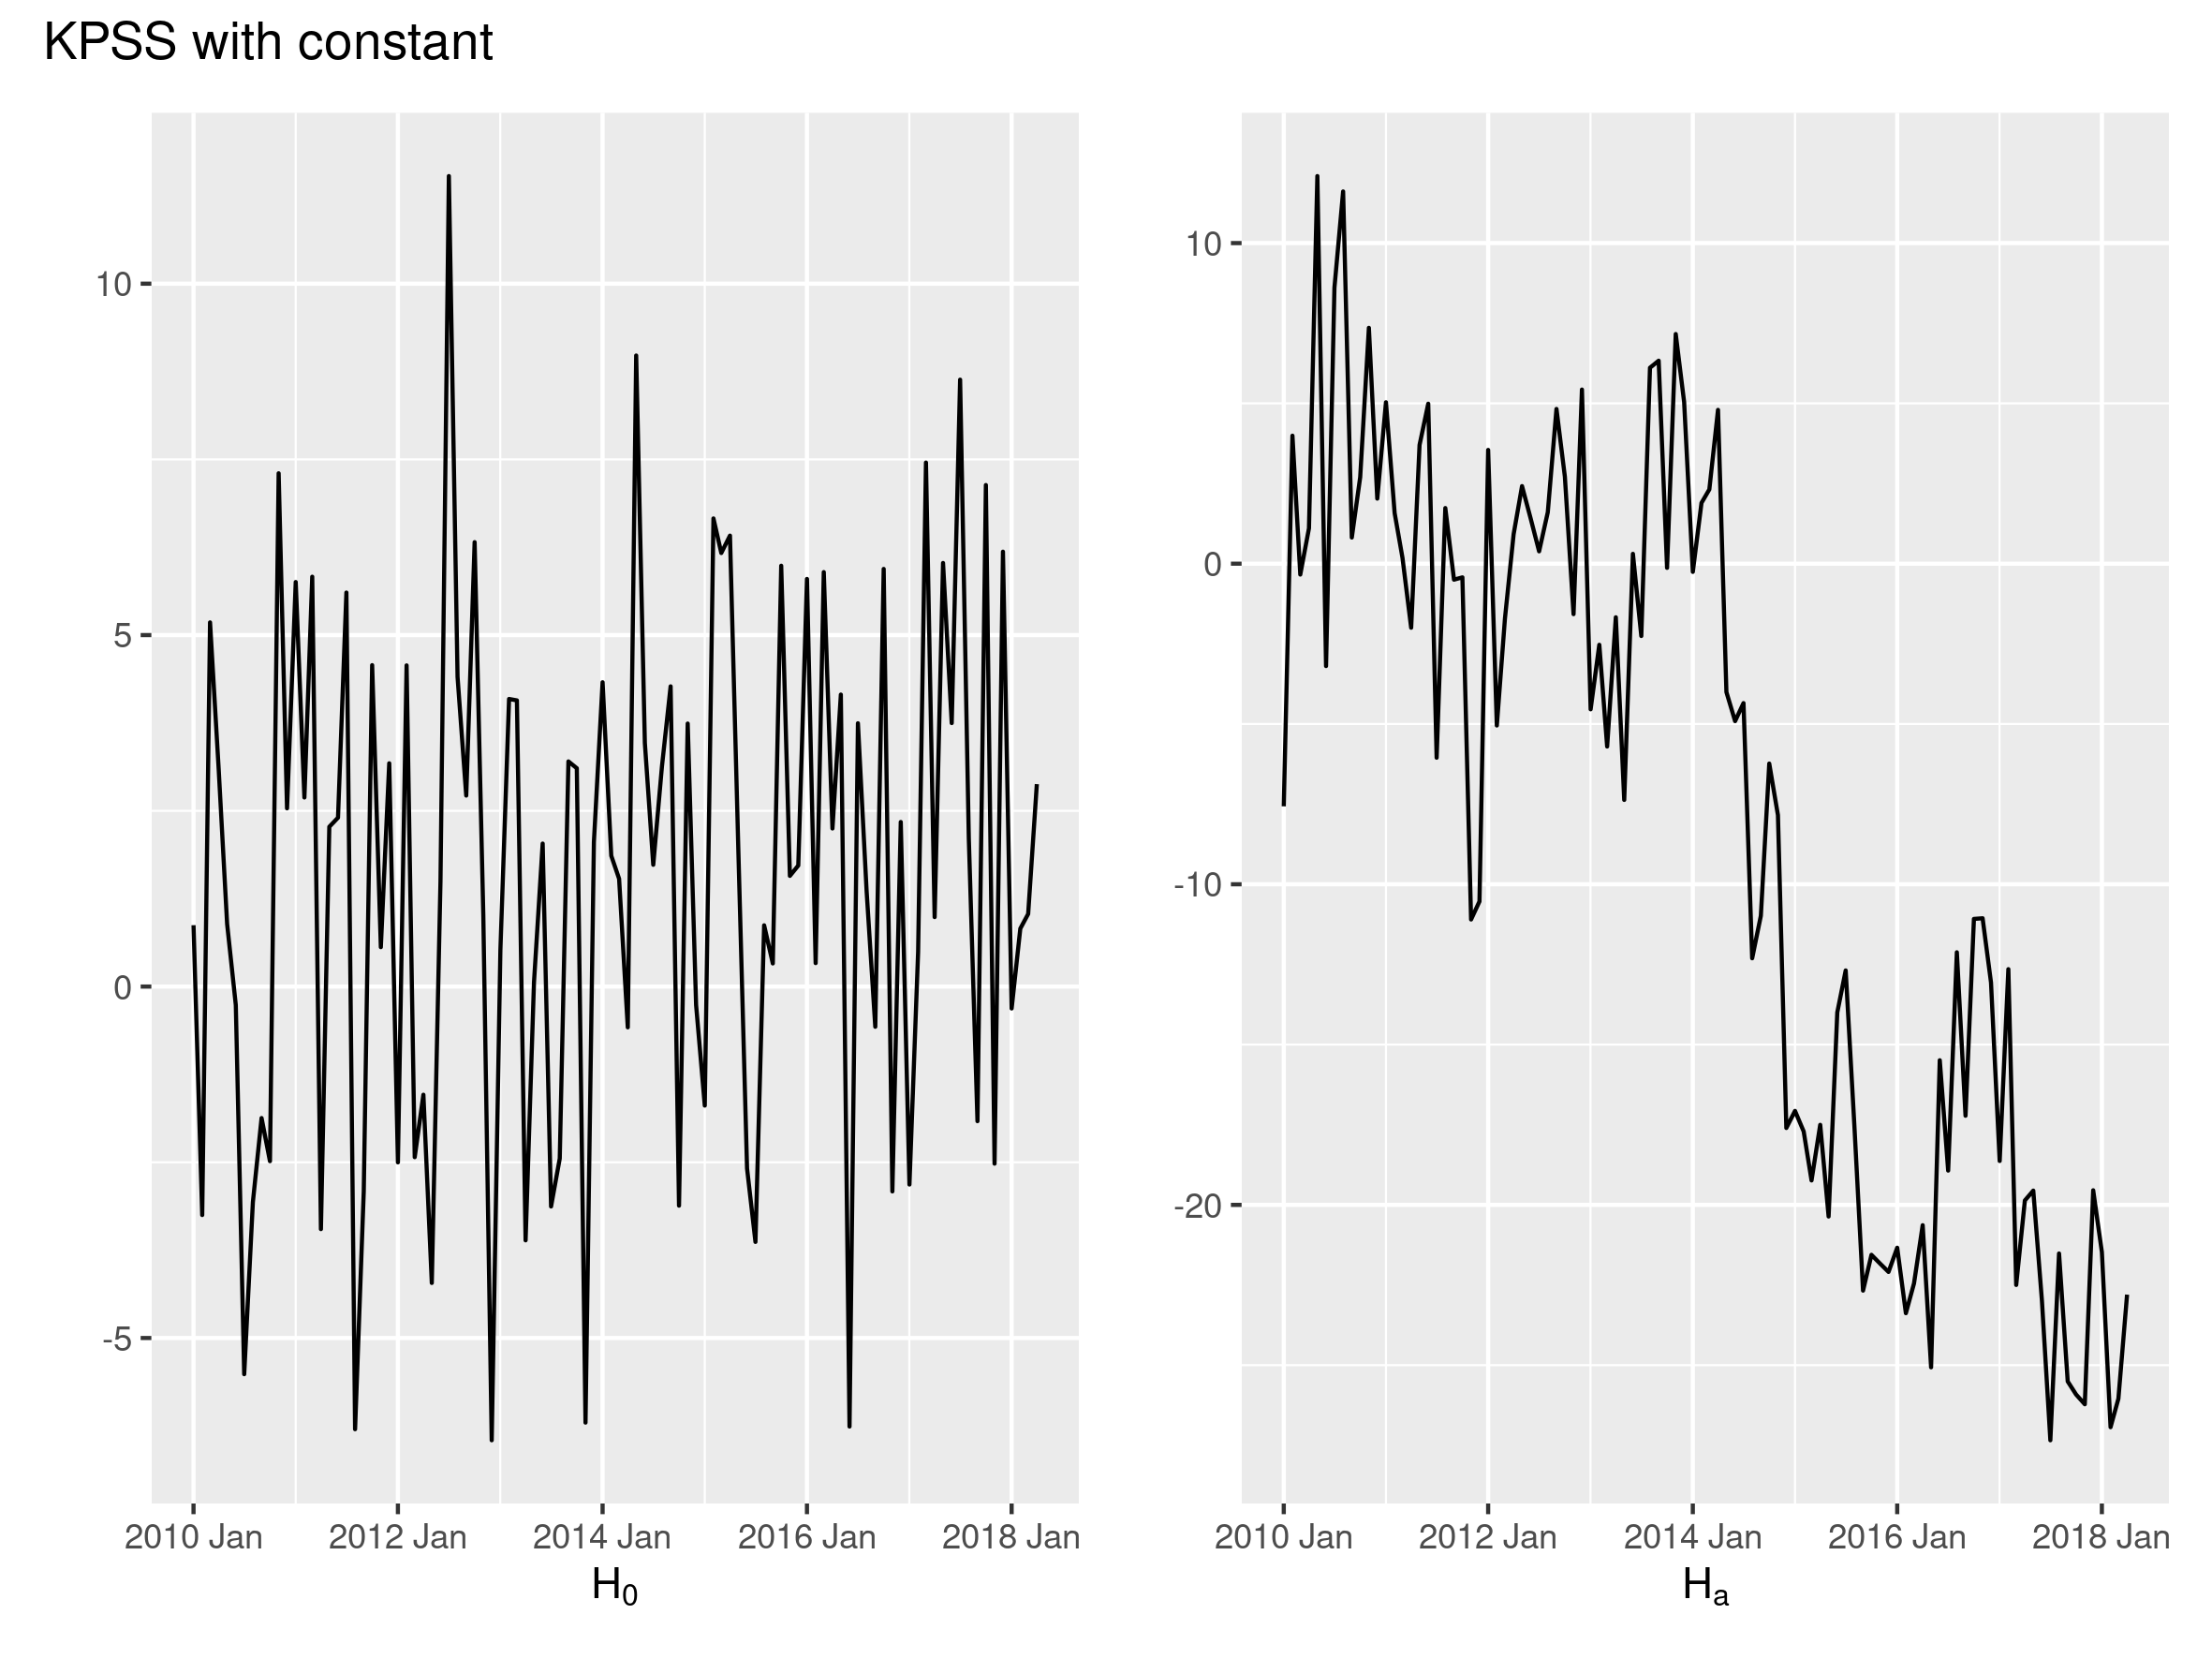
\includegraphics[width=\textwidth]{pictures/om_ts_06-077.png}
	
\end{frame}

\begin{frame}
	\frametitle{KPSS with constant: algorithm}
	
	Step 1. Evaluate regression on a \alert{constant }
	\[
	\widehat{y_t} = \hat c
	\]
	
	\pause
	Step 2. Calculate $KPSS$ statistics
	\[
	KPSS = \frac{\sum_{t=1}^T S_t^2}{T^2 \hat \lambda^2},
	\]
	where $S_t$ is the accumulated sum of residuals, $S_t = \hat u_1 + \ldots + \hat u_t$,
	
	and $\hat\lambda^2$ is a consistent estimator of the long-term variance.
	
	\pause
	Under true $H_0$, the distribution of the $KPSS$-statistic converges to a  \alert{special distribution} with $KPSS^c$!
	
	\pause
	Step 3. We conclude:
	
	If $KPSS > KPSS^c$ then $H_0$ is rejected
	
\end{frame}


\begin{frame}
	\frametitle{KPSS with trend}
	\[
	y_t = c + bt + rw_t + x_t,
	\]
	
	\pause
	
	\alert{$H_0$: $rw_t = 0$}
	
	$(x_t)$ is a stationary process with $\E(x_t) = 0$;
	
	\pause
	
	\alert{$H_a$: $rw_t = rw_{t-1} + u_t$}
	
	$rw_0 = 0$;
	
	$(x_t)$ is a stationary process with $\E(x_t) = 0$;
	
	$(u_t)$ is white noise independent of $(x_t)$
	
	\pause
	
	The first step of the algorithm will have a regression \alert{on a constant and a trend} and the statistic under null will have   another special distribution $KPSS^{ct}$
	
\end{frame}


\begin{frame}
	\frametitle{KPSS with trend: $H_0$ and $H_a$}
	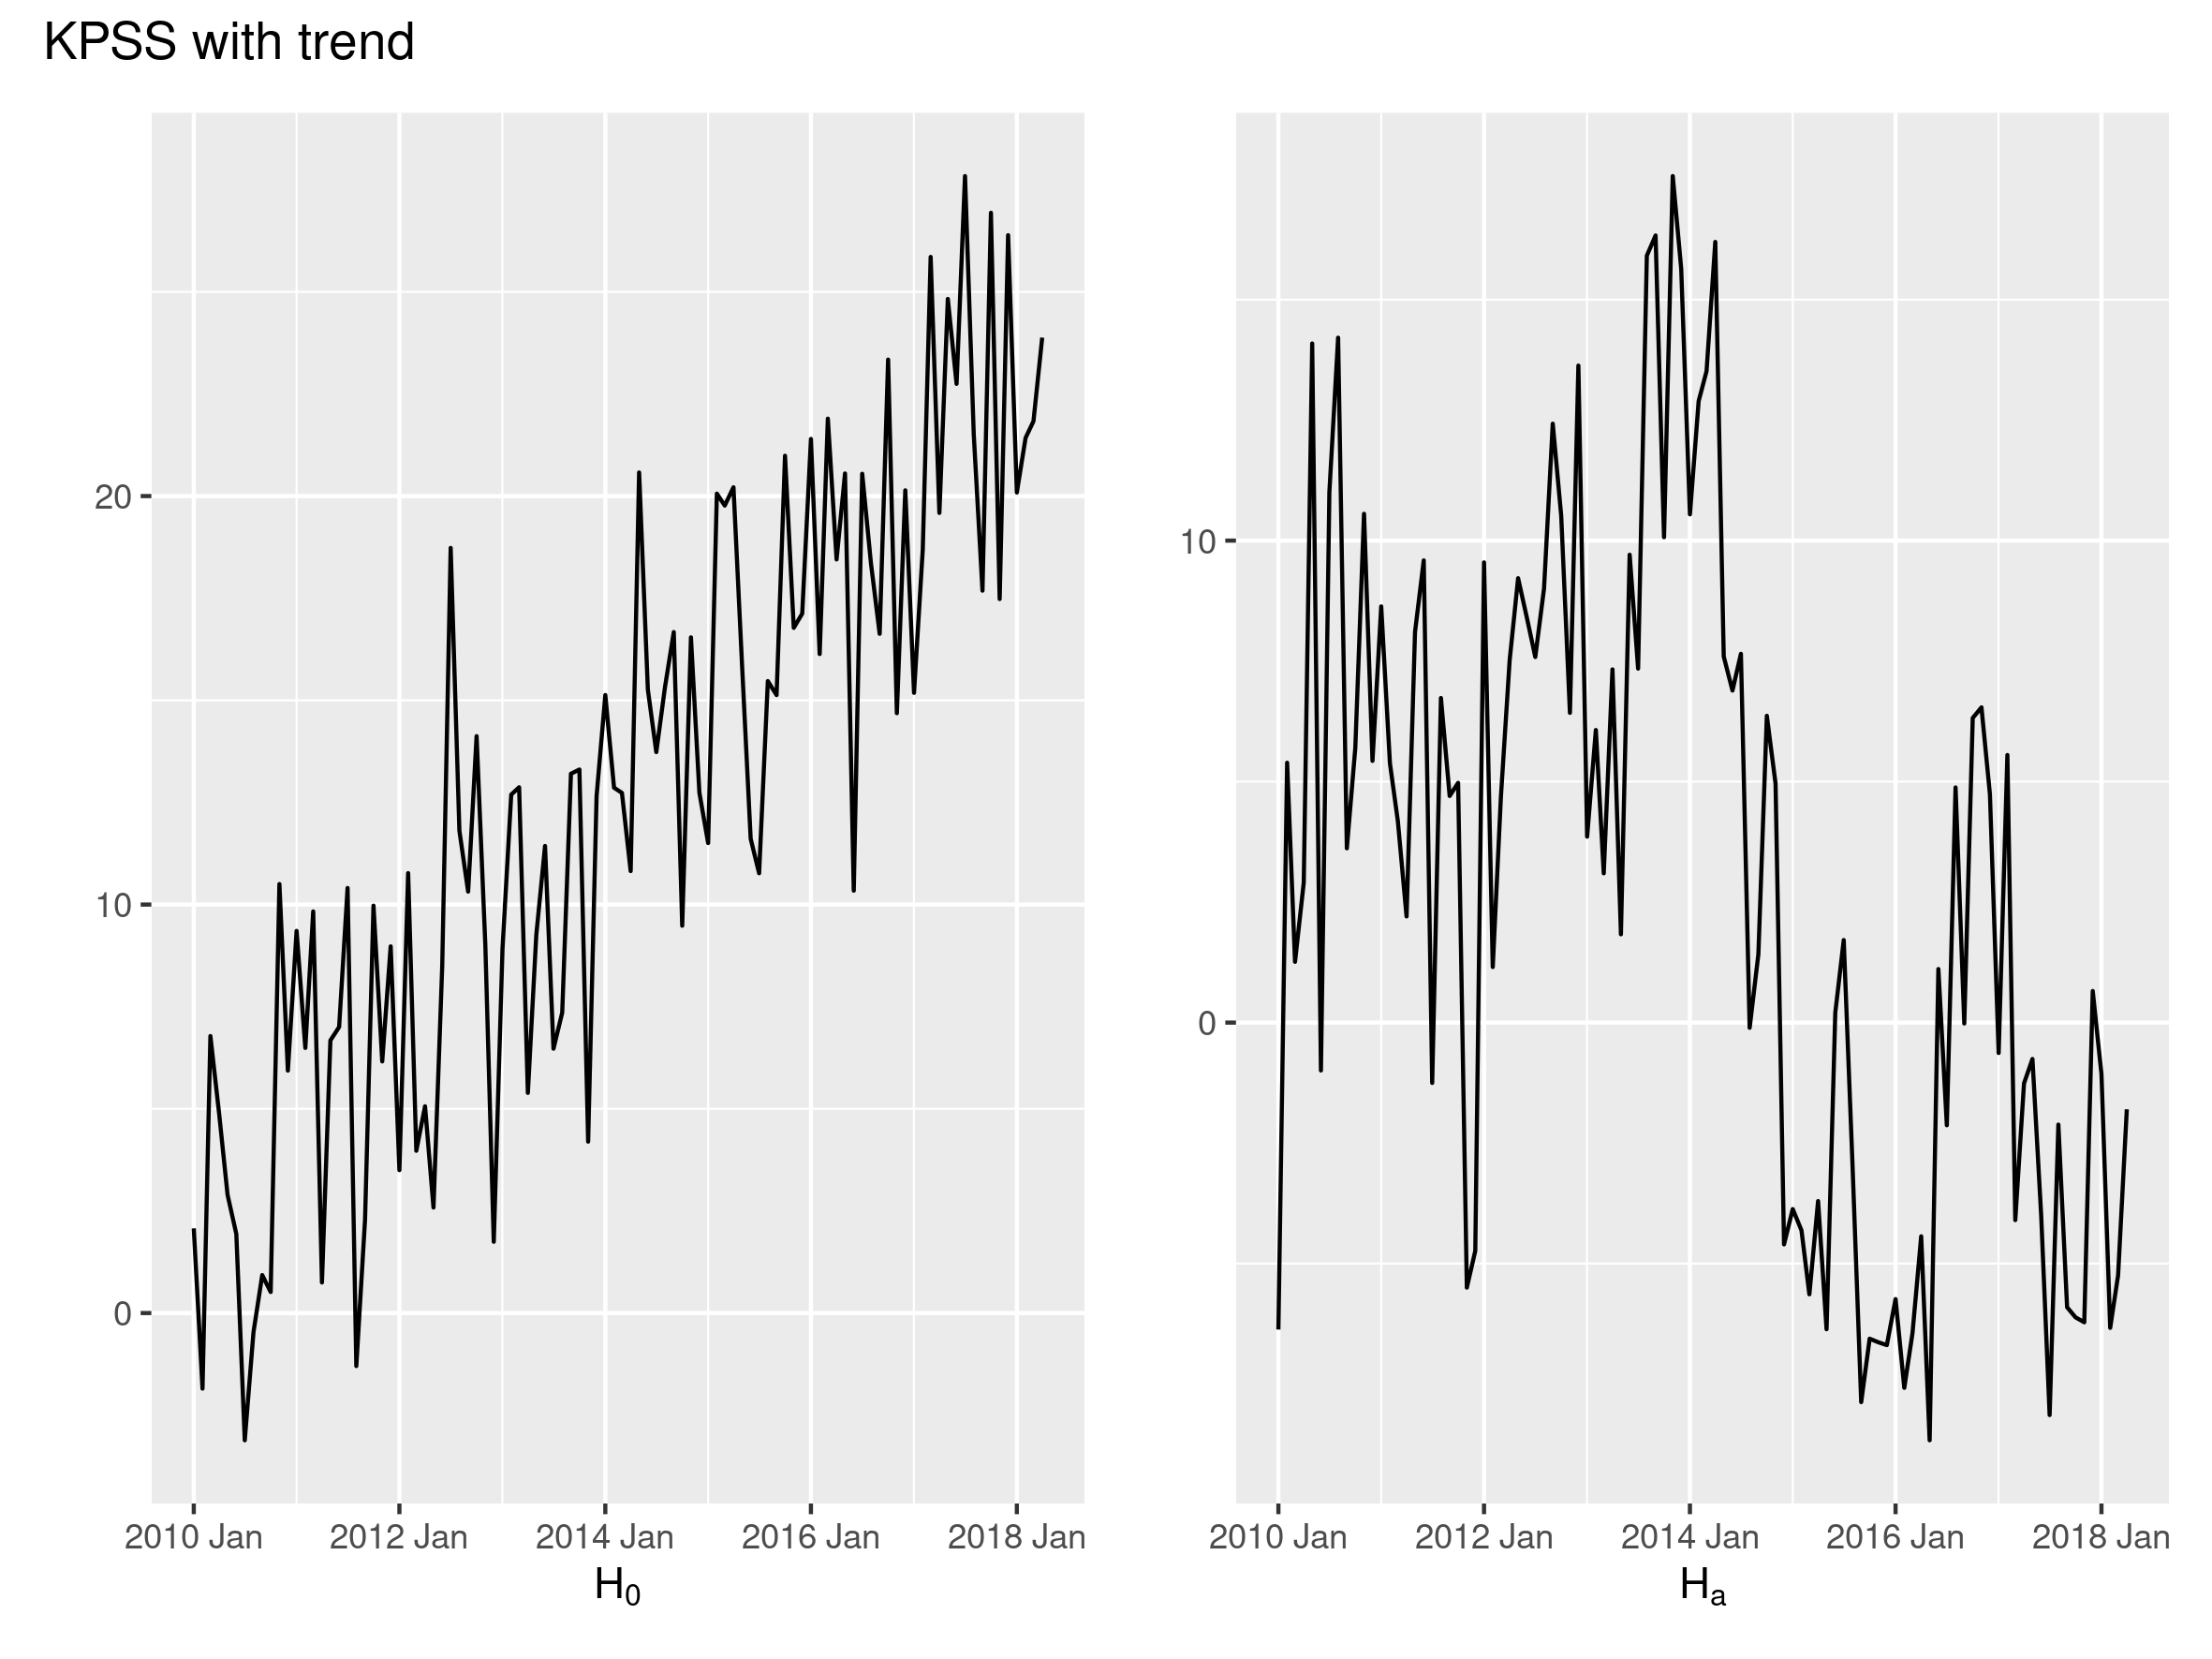
\includegraphics[width=\textwidth]{pictures/om_ts_06-086.png}
\end{frame}

% TODO: move A and B and highlight with color!
\begin{frame}
	\frametitle{Terminology}
	\[
	A. \quad y_t = a + bt + x_t
	\]
	
	$(y_t)$ — \alert{trend stationary} (stationary around the trend)
	
	$(x_t)$ — a stationary process with $\E(x_t) = 0$
	
	\pause Recipe: Estimate regression $a + bt$ with $ARMA$ errors for $(y_t)$.
	\pause
	\[
	B. \quad y_t = a + \sum_{i=1}^t x_i \text{ or } y_t = a + bt + \sum_{i=1}^t x_i
	\]
	
	$(x_t)$ — a stationary process with $\E(x_t) = 0$
	
	$(y_t)$ — \alert{difference stationary} (stationary in differences)
	
	\pause Recipe: evaluate $ARMA$ for $(\Delta y_t)$.
	
	\pause Both $(y_t)$ are non-stationary!
	
\end{frame}



\begin{frame}{KPSS test: Summary}
	
	\begin{itemize}[<+->]
		\item Applicable for making a decision about the transition to $\Delta y_t$
		\item Two versions of the KPSS test with different assumptions	
		
	\end{itemize}
\end{frame}



